%********************************************************************
% Appendix
%*******************************************************
% If problems with the headers: get headings in appendix etc. right
\markboth{\spacedlowsmallcaps{Appendices}}{\spacedlowsmallcaps{Appendices}}
%\chapter{Source Code Listings}

% TODO: Render source code with some other tool and include as a figure. This is breaking LaTeX.

%\section{Paragraph Splitter}
%\label{app:parsplitter}
%\subsection{ParSplitter.java}
%\lstinputlisting[nolol,language=Java,tabsize=4,stringstyle=\color{blue},basicstyle=\ttfamily\scriptsize]{../JSReflow/ParSplitter/src/ParSplitter.java}

%\newpage

\cleardoublepage
\chapter{A Sample Malleable Document}
\label{app:sampledoc}

This is the full rendering of a reasonably short document (the Wikipedia entry for The Butterley Company: see \url{http://en.wikipedia.org/wiki/Butterley_Company}). It contains three galley renderings, and has ordered dictionaries both for words, and for position deltas.

\section{butterley.html}
\emph{the \textsc{html} page within which the document is displayed}
%\lstinputlisting[nolol,language=html,tabsize=4,stringstyle=\color{blue},basicstyle=\ttfamily\scriptsize]{../JSReflow/butterley.html}

\section{style.css}
\emph{generic formatting instructions for the document}
%\lstinputlisting[nolol,tabsize=4,stringstyle=\color{blue},basicstyle=\ttfamily\scriptsize]{../JSReflow/styles.css}
\newpage

\section{script-json-rel.js}
\emph{the script used to perform the layout at view-time}
%\lstinputlisting[nolol,language=c,tabsize=4,stringstyle=\color{blue},basicstyle=\ttfamily\scriptsize]{../JSReflow/script-json-rel.js}

\newpage

\section{butterley.js}
\emph{the layout data of the document itself}
%\lstinputlisting[nolol,language=c,tabsize=4,stringstyle=\color{blue},basicstyle=\ttfamily\tiny]{..//JSReflow/butterley.js}

\cleardoublepage
\chapter{Sample Layouts}
\label{app:layouts}
\begin{figure}
\begin{center}
\fbox{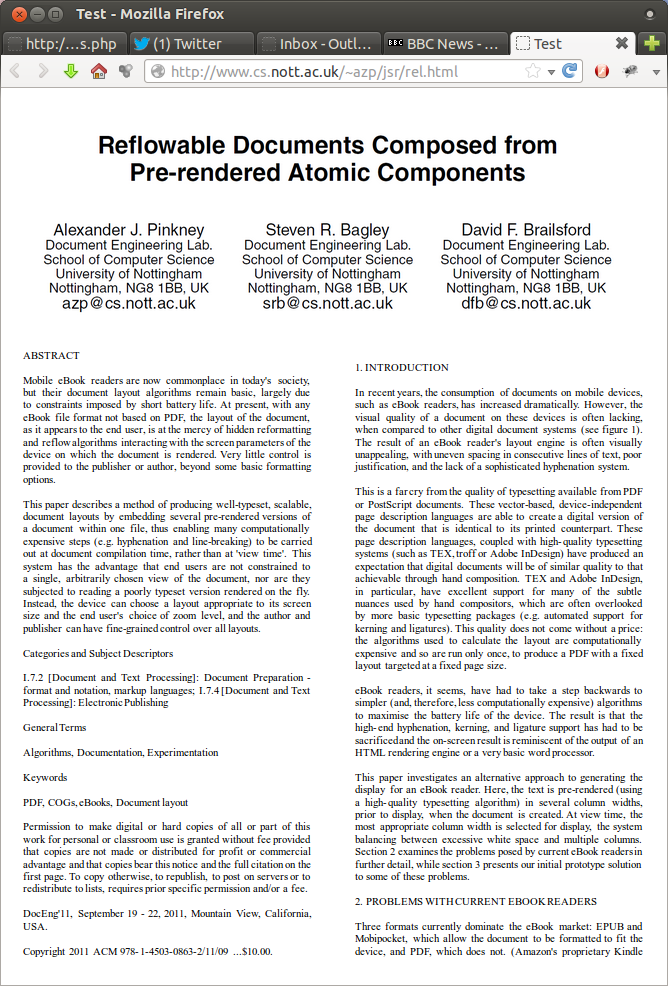
\includegraphics[trim=0in 0in 0in 1.2in, clip=true, width=0.47\textwidth]{gfx/p1}}\hspace{0.01\textwidth}
\fbox{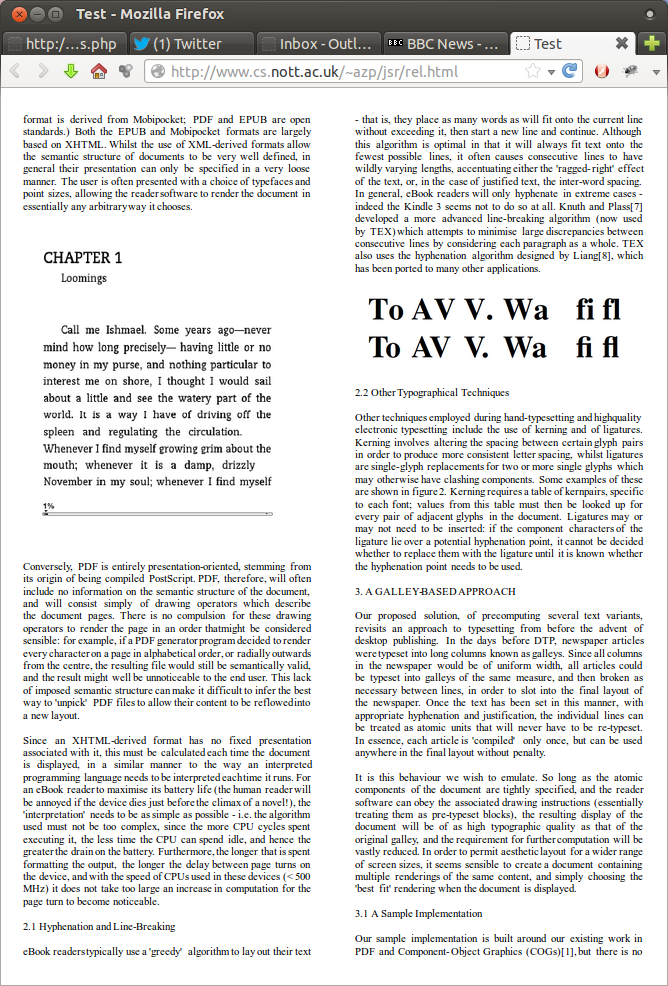
\includegraphics[trim=0in 0in 0in 1.2in, clip=true, width=0.47\textwidth]{gfx/p2}}

\vspace{0.2in}
\fbox{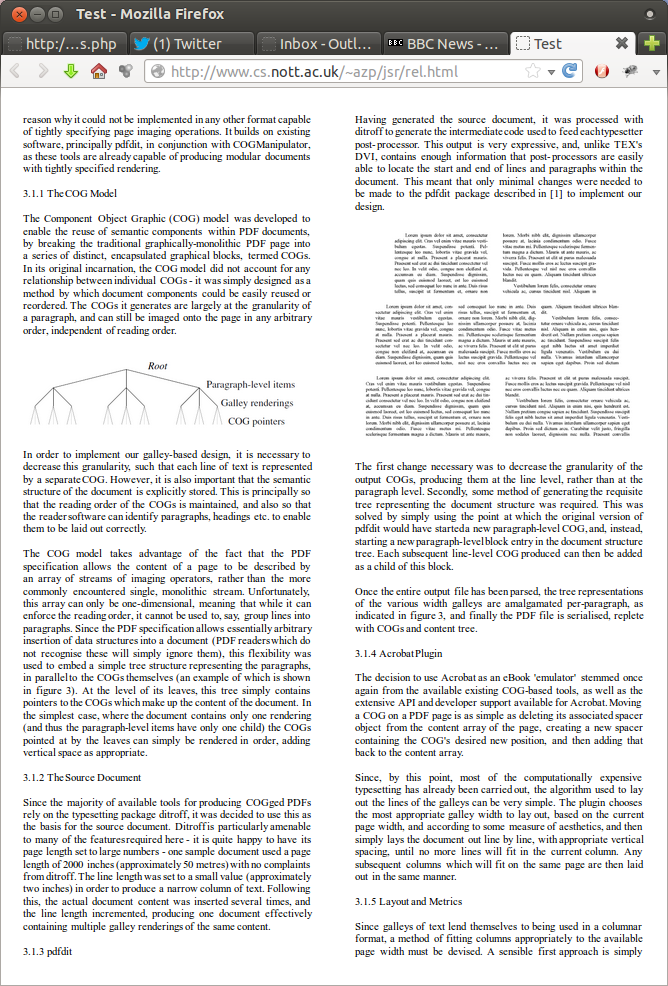
\includegraphics[trim=0in 0in 0in 1.2in, clip=true, width=0.47\textwidth]{gfx/p3}}\hspace{0.01\textwidth}
\fbox{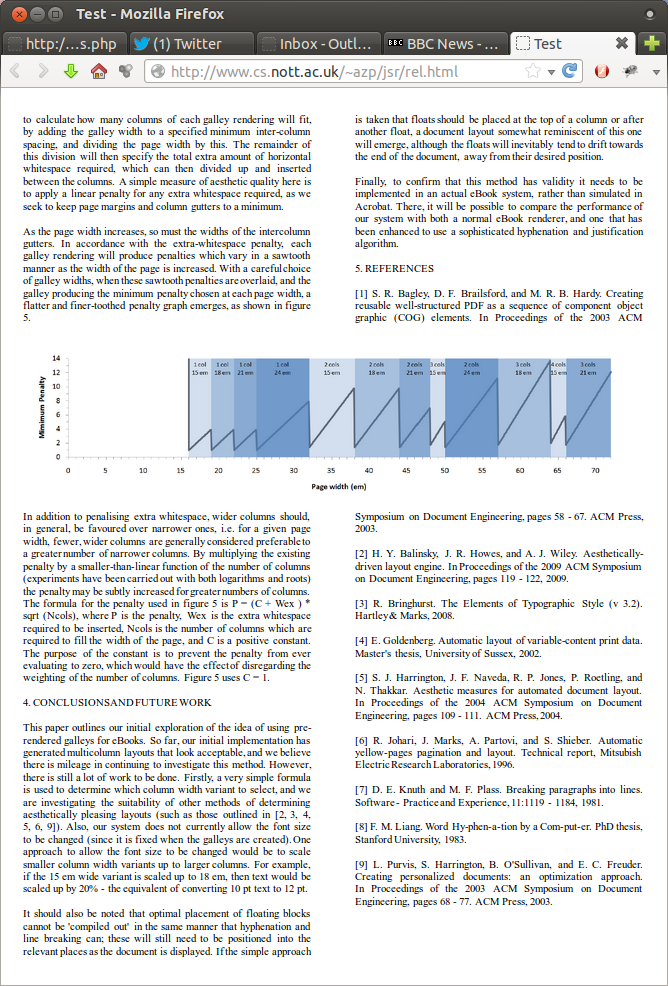
\includegraphics[trim=0in 0in 0in 1.2in, clip=true, width=0.47\textwidth]{gfx/p4}}
\end{center}
\caption[A sample of document layout]{\cite{Pinkney2011} laid out by the malleable document system, running in Mozilla Firefox. The page size has been selected to resemble that of A4 paper in a portrait orientation.}
\label{fig:example-portrait}
\end{figure}

\begin{sidewaysfigure}
\begin{center}
\fbox{
\includegraphics[trim=0in 0in 0in 1.2in, clip=true, width=0.45\textwidth]{gfx/q1}}\hspace{0.05\textwidth}
\fbox{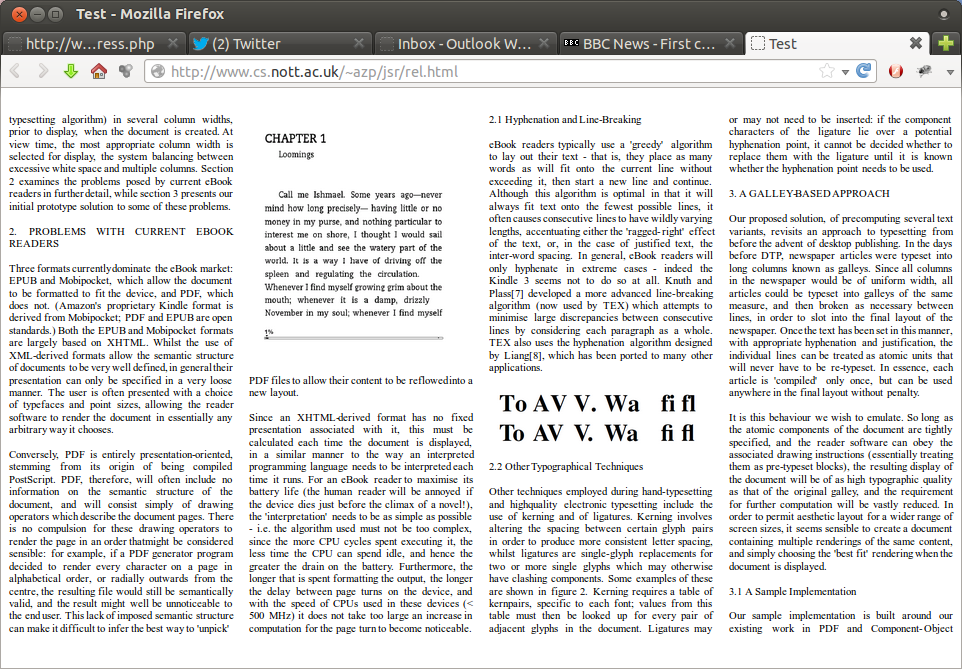
\includegraphics[trim=0in 0in 0in 1.2in, clip=true, width=0.45\textwidth]{gfx/q2}}

\vspace{0.2in}
\fbox{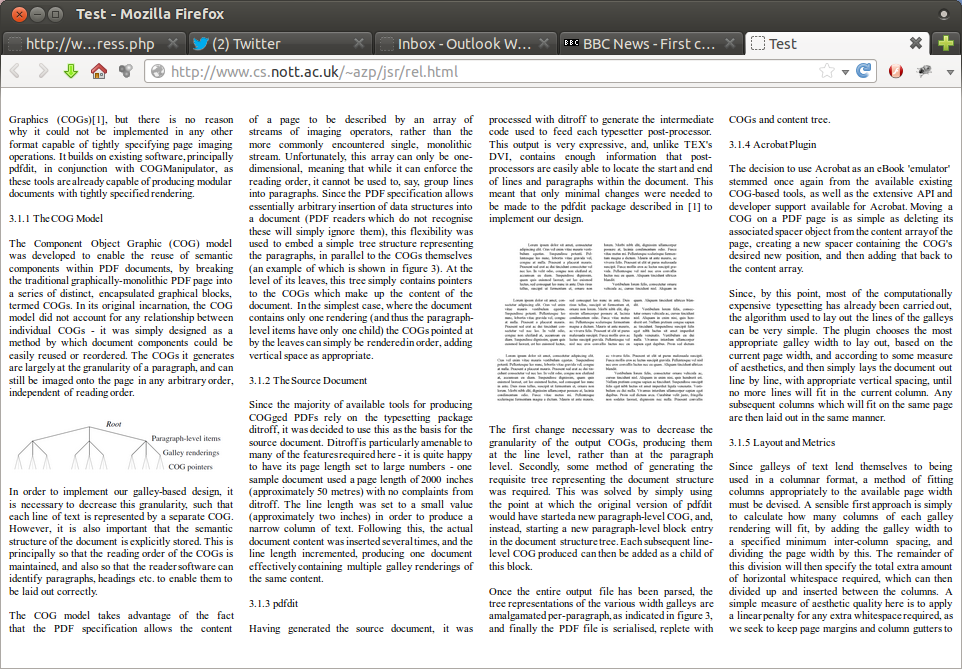
\includegraphics[trim=0in 0in 0in 1.2in, clip=true, width=0.45\textwidth]{gfx/q3}}\hspace{0.05\textwidth}
\fbox{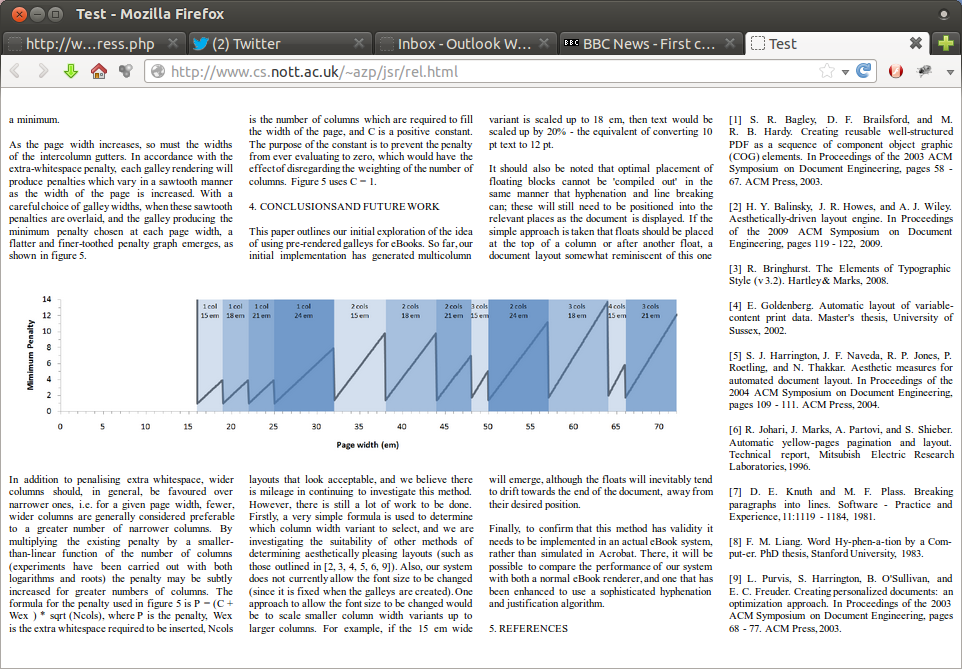
\includegraphics[trim=0in 0in 0in 1.2in, clip=true, width=0.45\textwidth]{gfx/q4}}
\end{center}
\caption[A sample of document layout]{\cite{Pinkney2011} laid out by the malleable document system, running in Mozilla Firefox. The page size has been selected to resemble that of A4 paper in a landscape orientation.}
\label{fig:example-landscape}
\end{sidewaysfigure}

\begin{figure}
\begin{center}
\newlength{\imgwid} \setlength{\imgwid}{0.29\textwidth}
\fbox{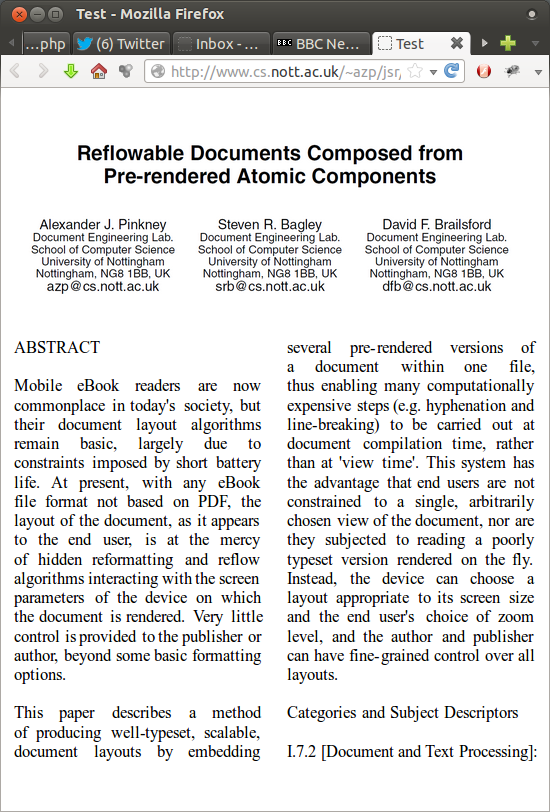
\includegraphics[trim=0in 0in 0in 1.2in, clip=true, width=\imgwid]{gfx/r1}}
\fbox{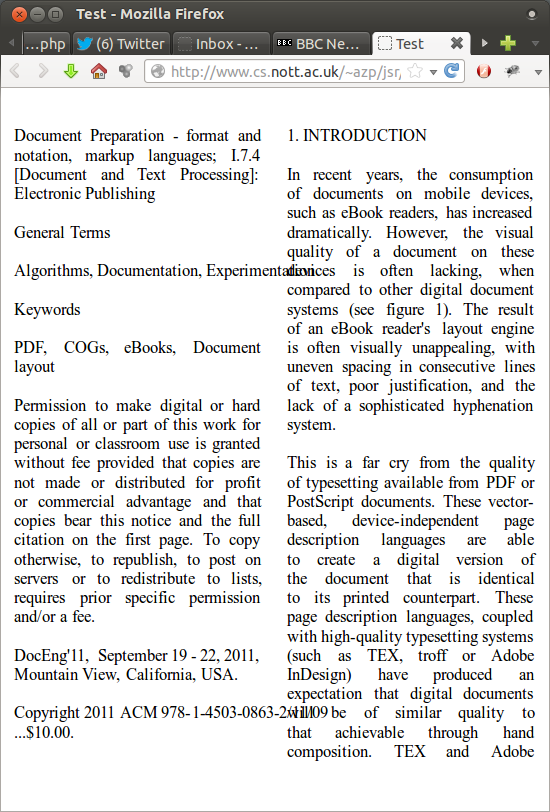
\includegraphics[trim=0in 0in 0in 1.2in, clip=true, width=\imgwid]{gfx/r2}}
\fbox{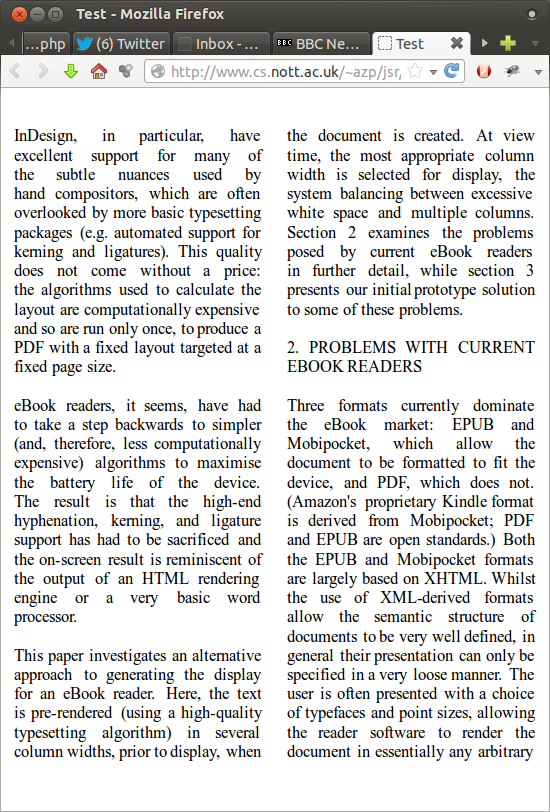
\includegraphics[trim=0in 0in 0in 1.2in, clip=true, width=\imgwid]{gfx/r3}}
\fbox{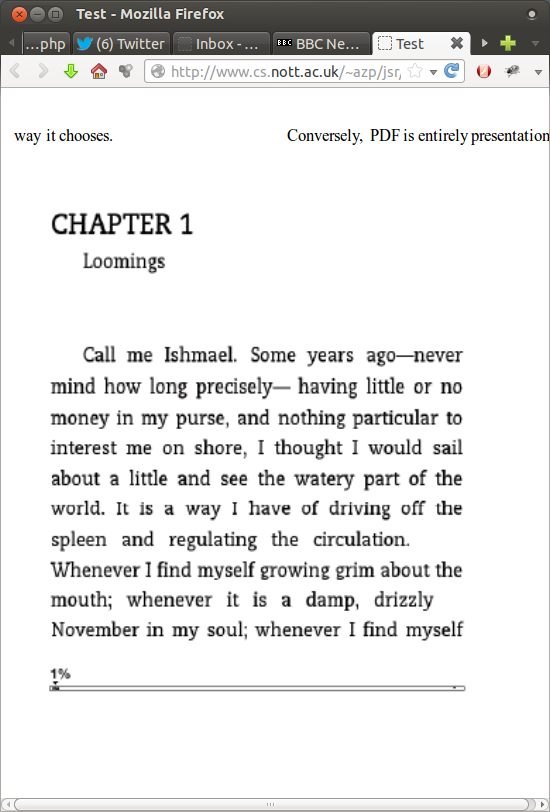
\includegraphics[trim=0in 0in 0in 1.2in, clip=true, width=\imgwid]{gfx/r4}}
\fbox{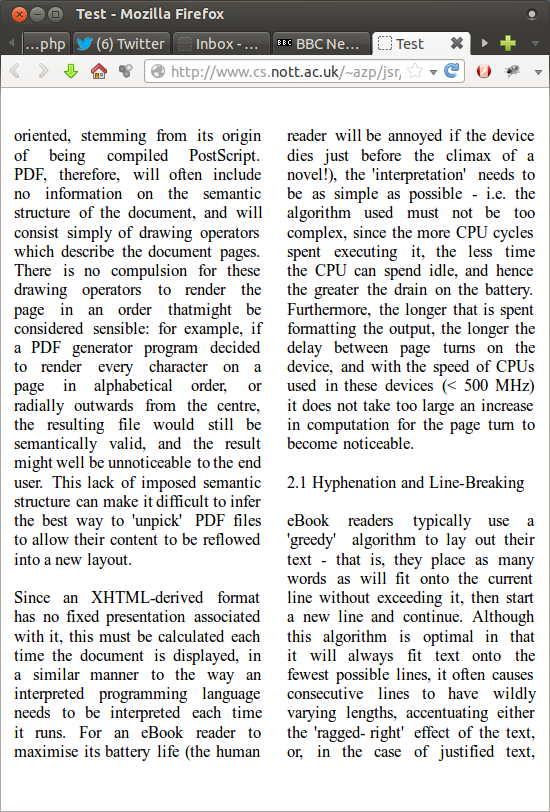
\includegraphics[trim=0in 0in 0in 1.2in, clip=true, width=\imgwid]{gfx/r5}}
\fbox{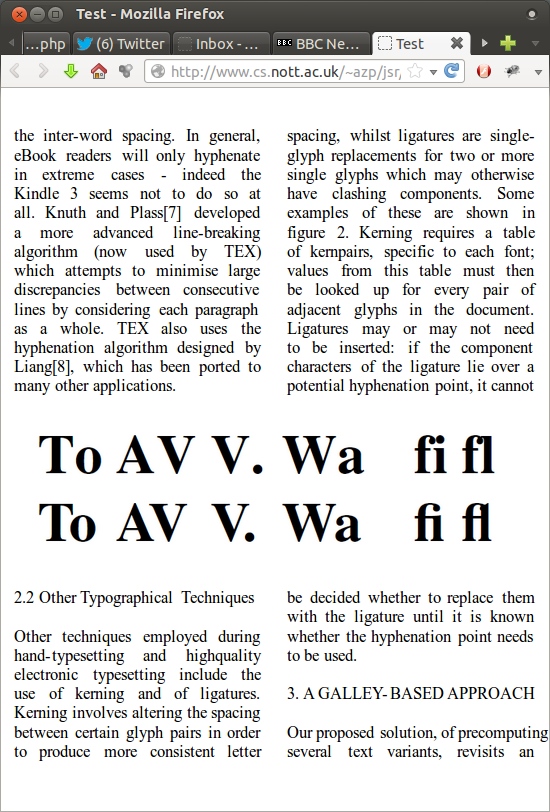
\includegraphics[trim=0in 0in 0in 1.2in, clip=true, width=\imgwid]{gfx/r6}}
\fbox{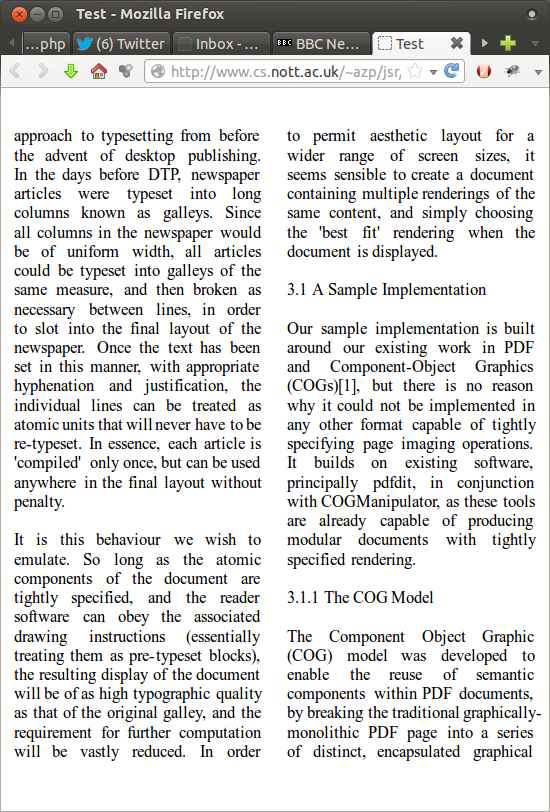
\includegraphics[trim=0in 0in 0in 1.2in, clip=true, width=\imgwid]{gfx/r7}}
\fbox{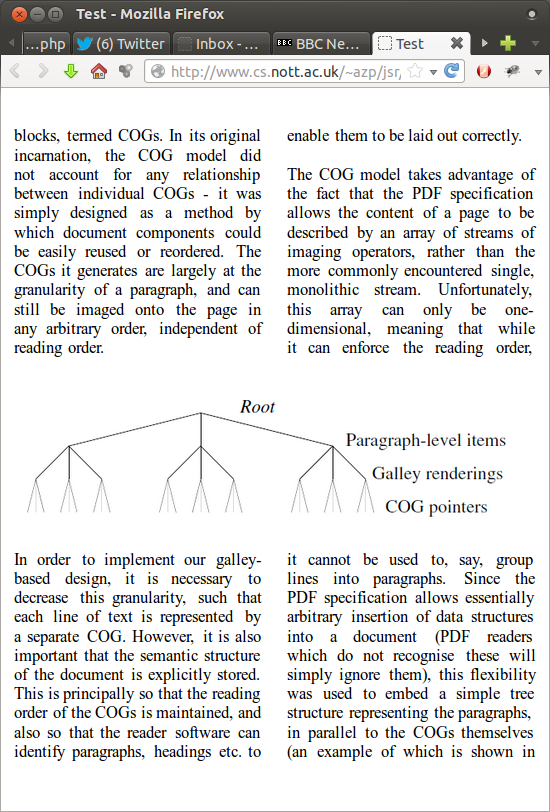
\includegraphics[trim=0in 0in 0in 1.2in, clip=true, width=\imgwid]{gfx/r8}}
\fbox{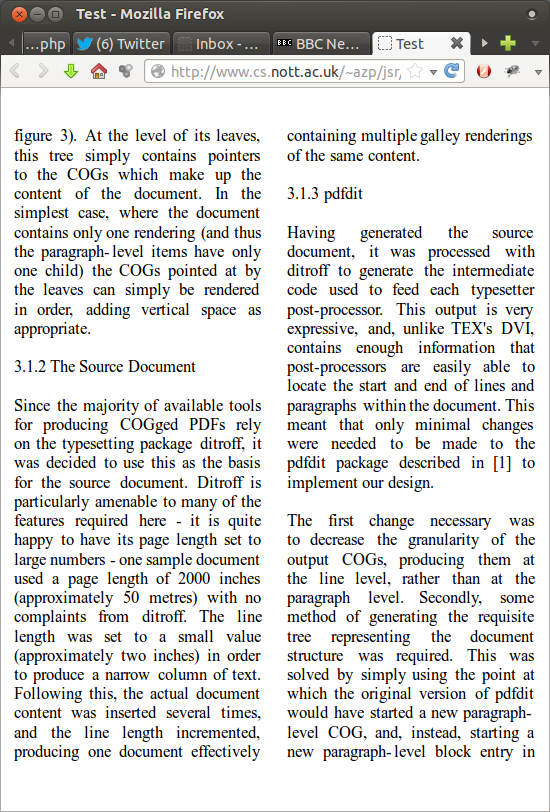
\includegraphics[trim=0in 0in 0in 1.2in, clip=true, width=\imgwid]{gfx/r9}}
\fbox{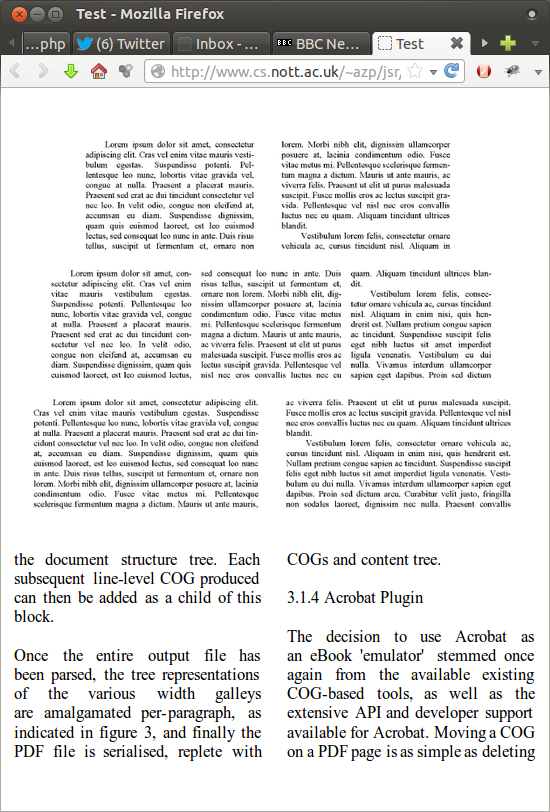
\includegraphics[trim=0in 0in 0in 1.2in, clip=true, width=\imgwid]{gfx/r10}}
\fbox{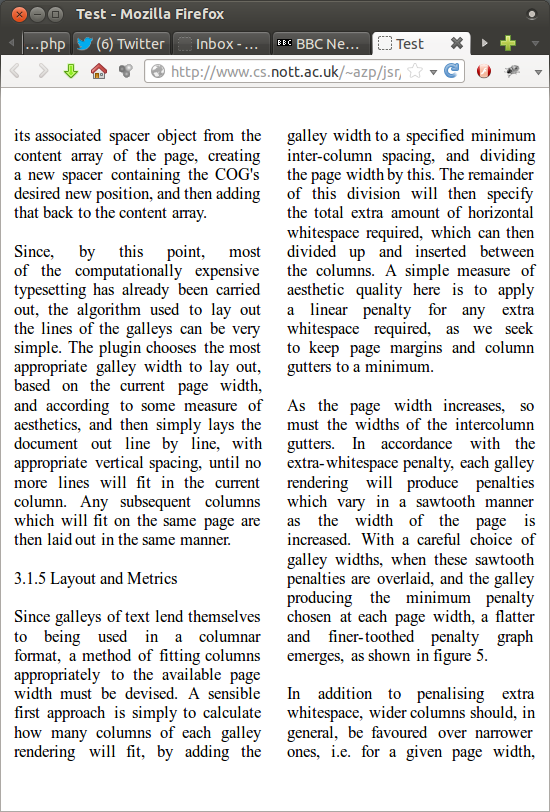
\includegraphics[trim=0in 0in 0in 1.2in, clip=true, width=\imgwid]{gfx/r11}}
\fbox{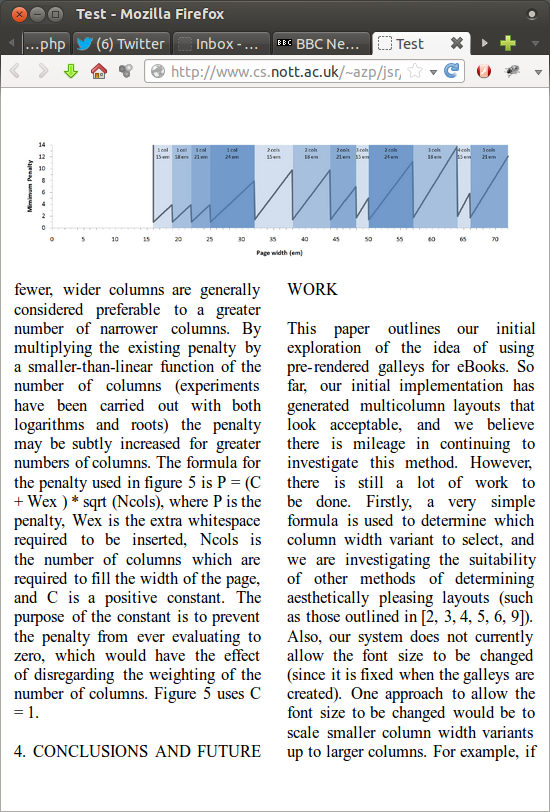
\includegraphics[trim=0in 0in 0in 1.2in, clip=true, width=\imgwid]{gfx/r12}}
\fbox{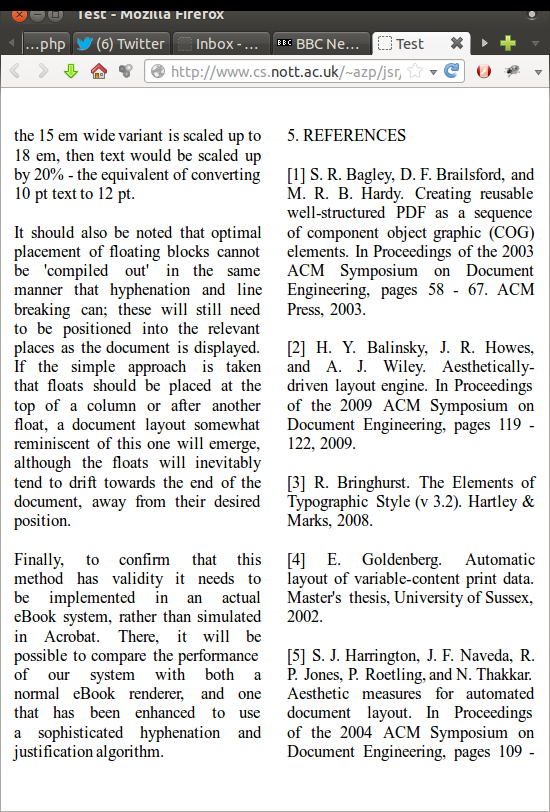
\includegraphics[trim=0in 0in 0in 1.2in, clip=true, width=\imgwid]{gfx/r13}}
\fbox{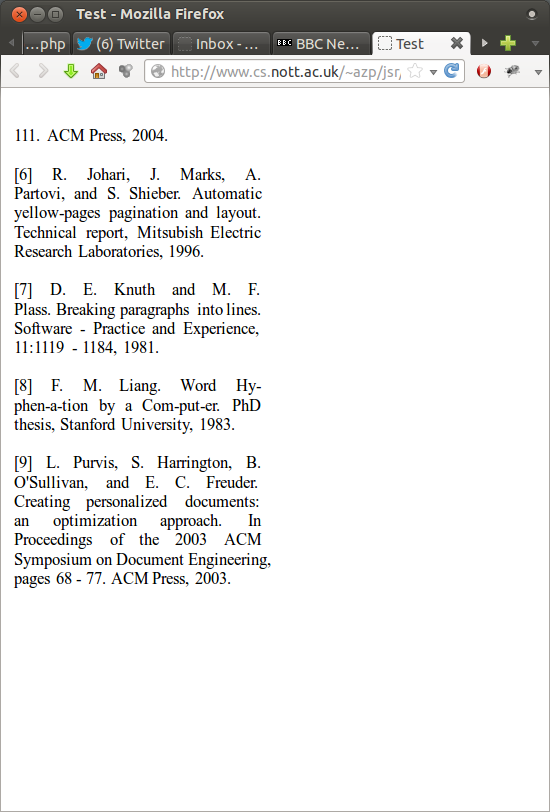
\includegraphics[trim=0in 0in 0in 1.2in, clip=true, width=\imgwid]{gfx/r14}}
\end{center}
\caption[A sample of document layout]{\cite{Pinkney2011} laid out by the malleable document system, running in Mozilla Firefox. The page size has been selected to resemble that of an \ebook{} reader in a portrait orientation.}
\label{fig:example-ereader}
\end{figure}

\begin{figure}
\begin{center}
\fbox{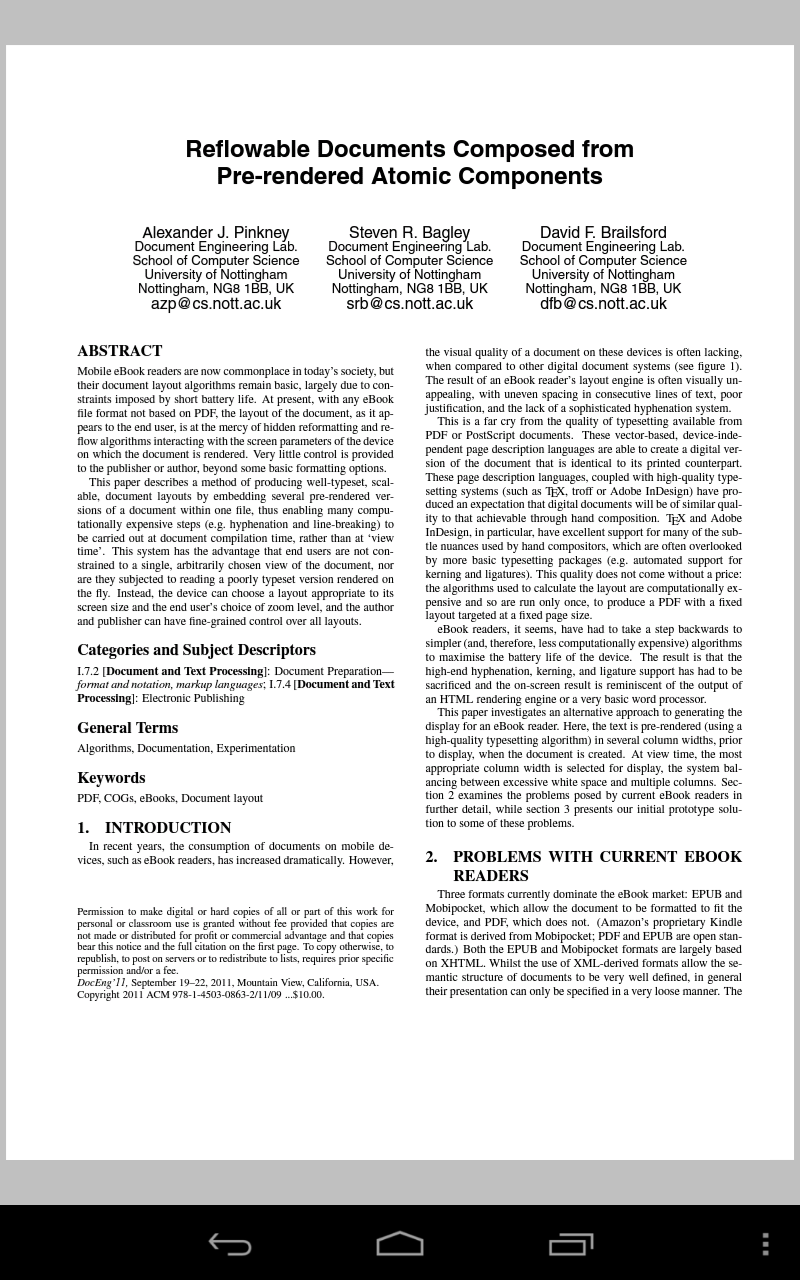
\includegraphics[trim=0.1in 2in 0.1in 1in, clip=true, width=0.47\textwidth]{gfx/pbb11-1}}\hspace{0.01\textwidth}
\fbox{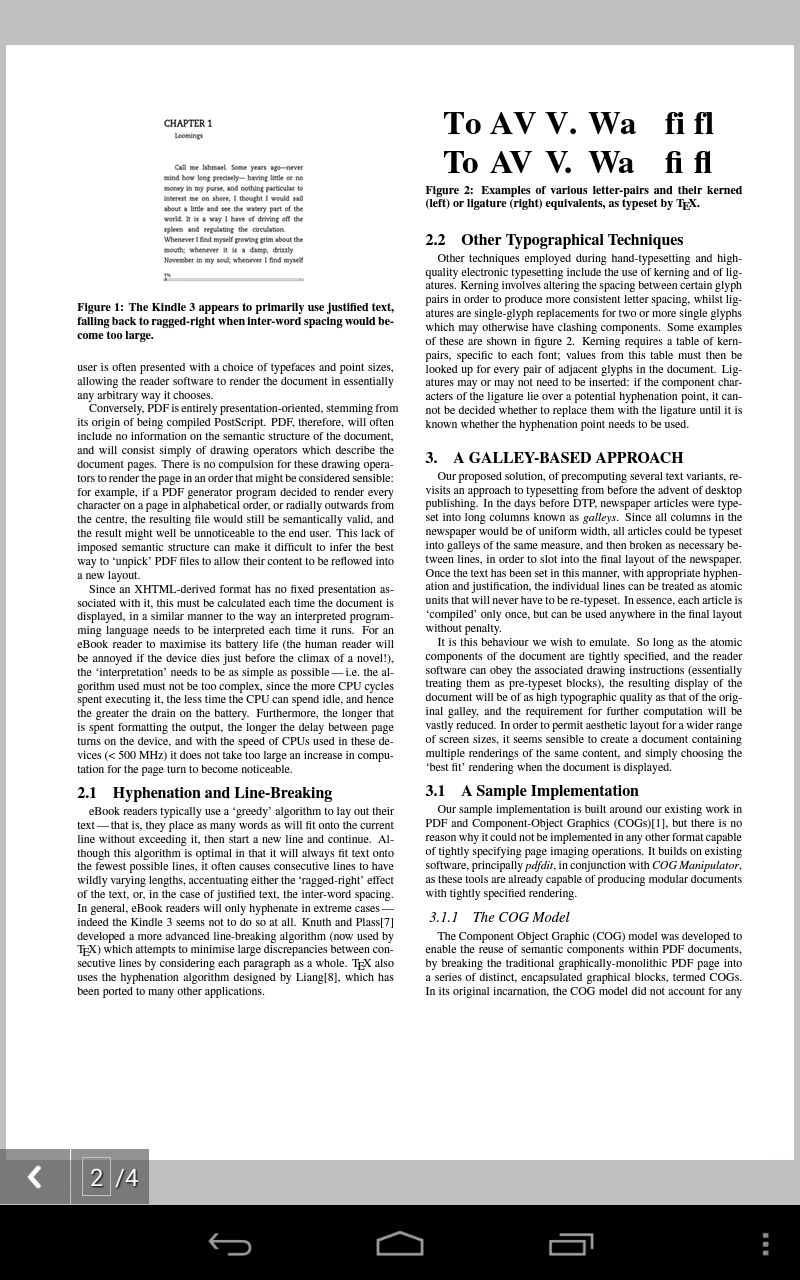
\includegraphics[trim=0.1in 2in 0.1in 1in, clip=true, width=0.47\textwidth]{gfx/pbb11-2}}

\vspace{0.2in}
\fbox{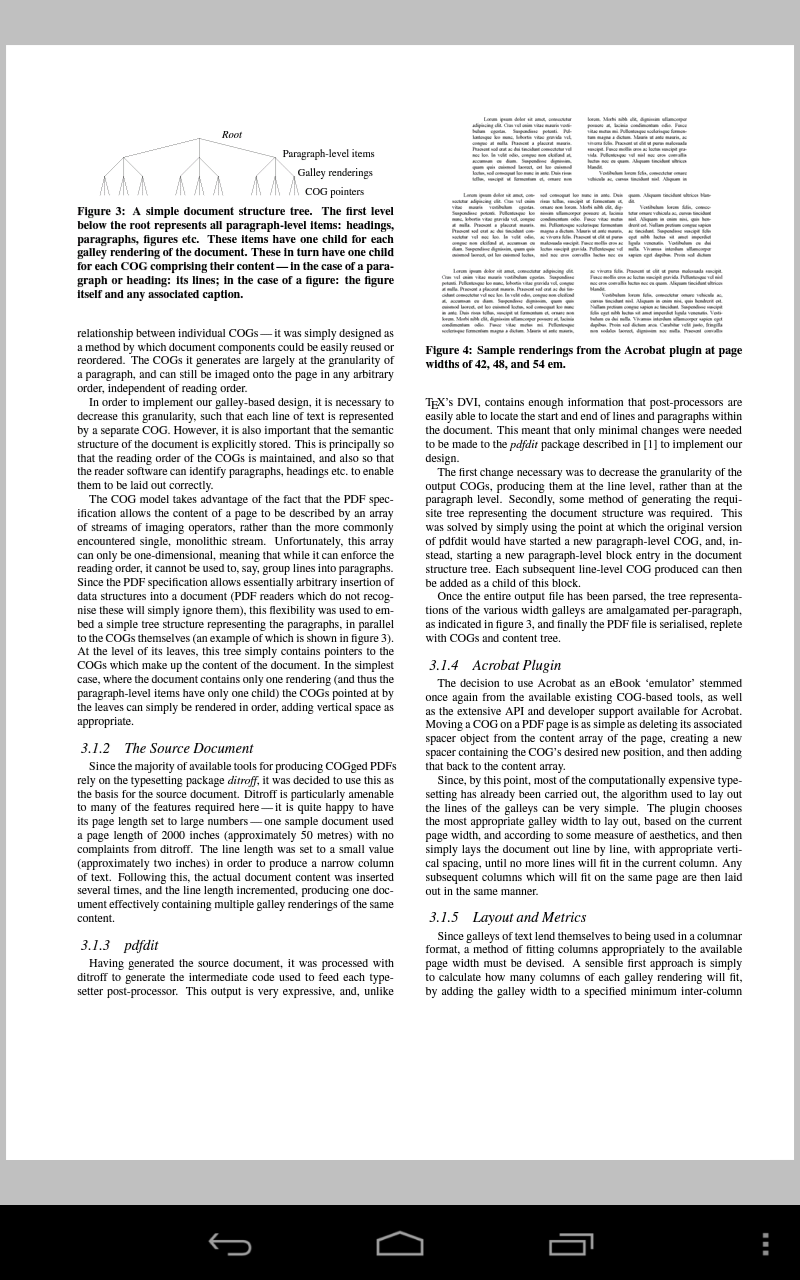
\includegraphics[trim=0.1in 2in 0.1in 1in, clip=true, width=0.47\textwidth]{gfx/pbb11-3}}\hspace{0.01\textwidth}
\fbox{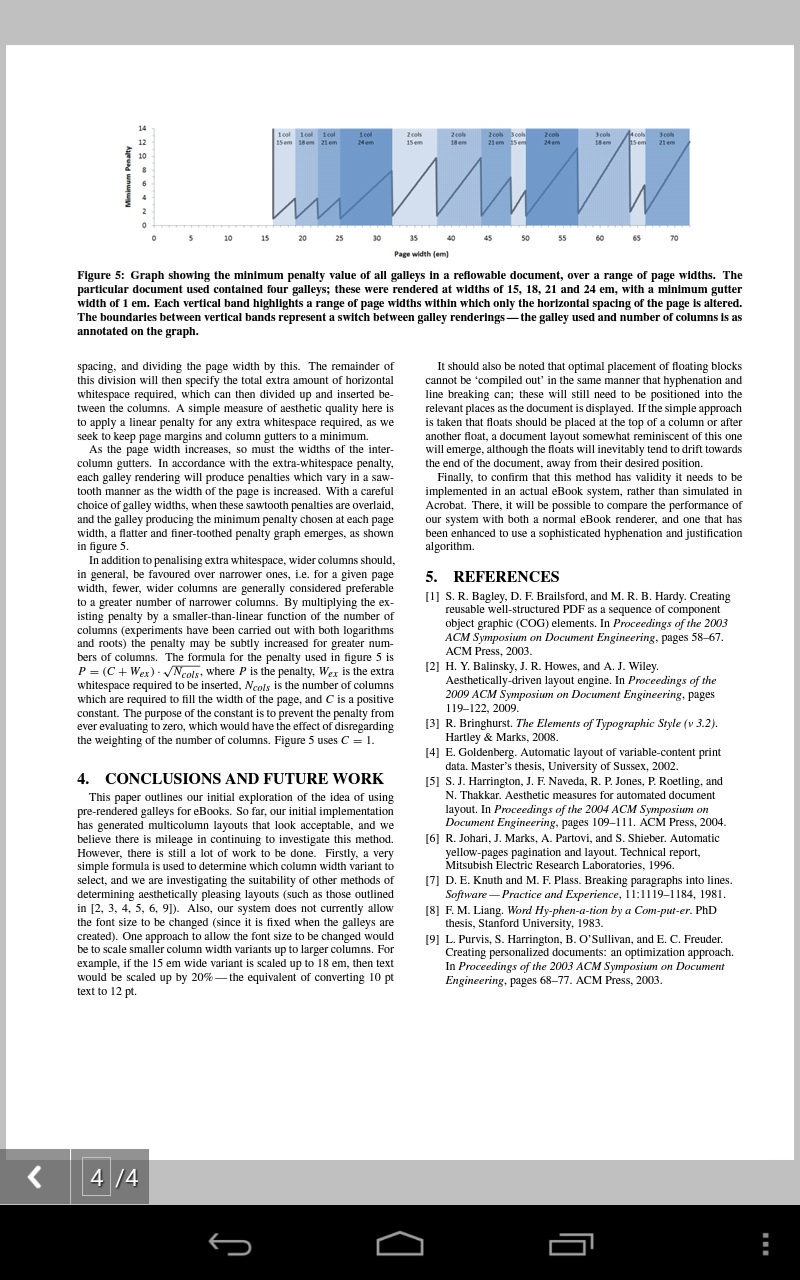
\includegraphics[trim=0.1in 2in 0.1in 1in, clip=true, width=0.47\textwidth]{gfx/pbb11-4}}
\end{center}
\caption[A document laid out by \LaTeX]{\cite{Pinkney2011} as rendered by \LaTeX. The layout is very similar to that shown in Figure~\ref{fig:example-portrait}, though \LaTeX{} favours placing floats at the top of columns, rather than directly at their logical position.}
\label{fig:example-latex}
\end{figure}

\begin{figure}
\begin{center}
\fbox{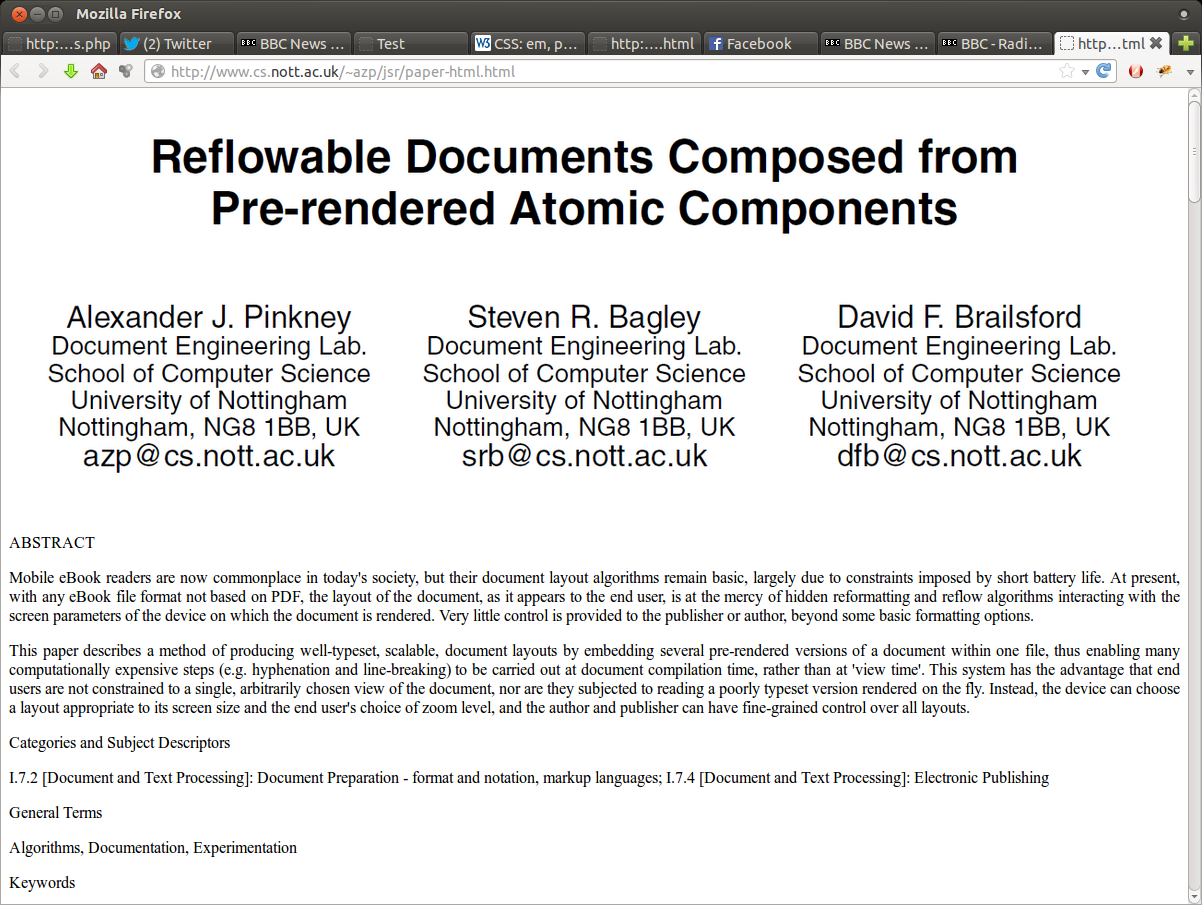
\includegraphics[trim=0in 0in 0in 1.2in, clip=true, width=0.47\textwidth]{gfx/html1}}\hspace{0.01\textwidth}
\fbox{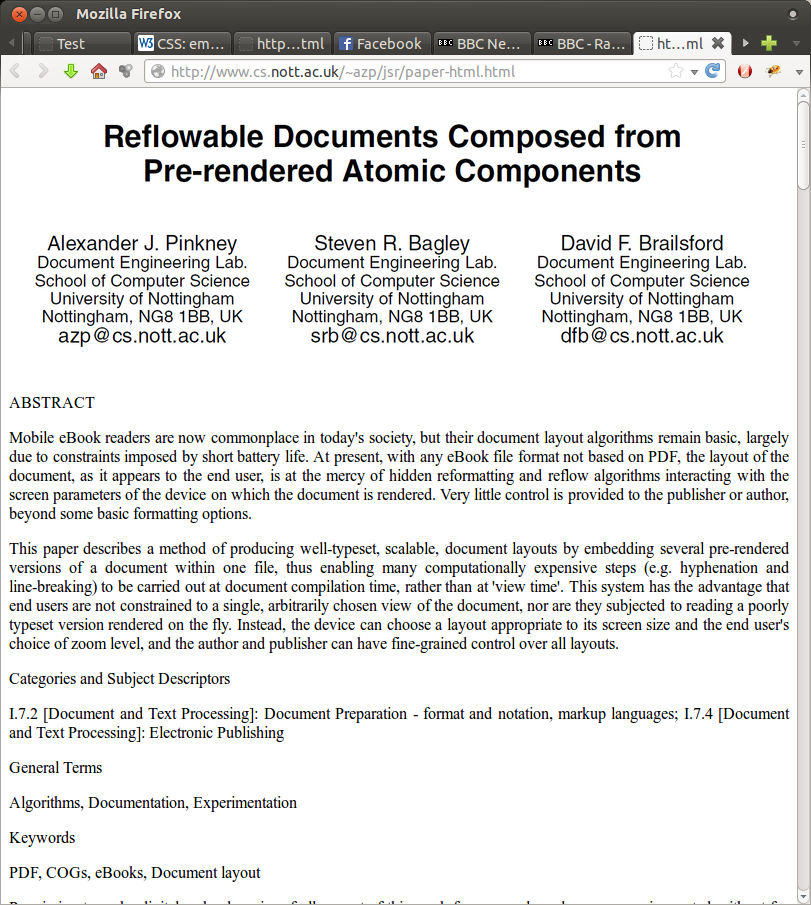
\includegraphics[trim=0in 0in 0in 1.2in, clip=true, width=0.47\textwidth]{gfx/html2}}

\vspace{0.2in}
\fbox{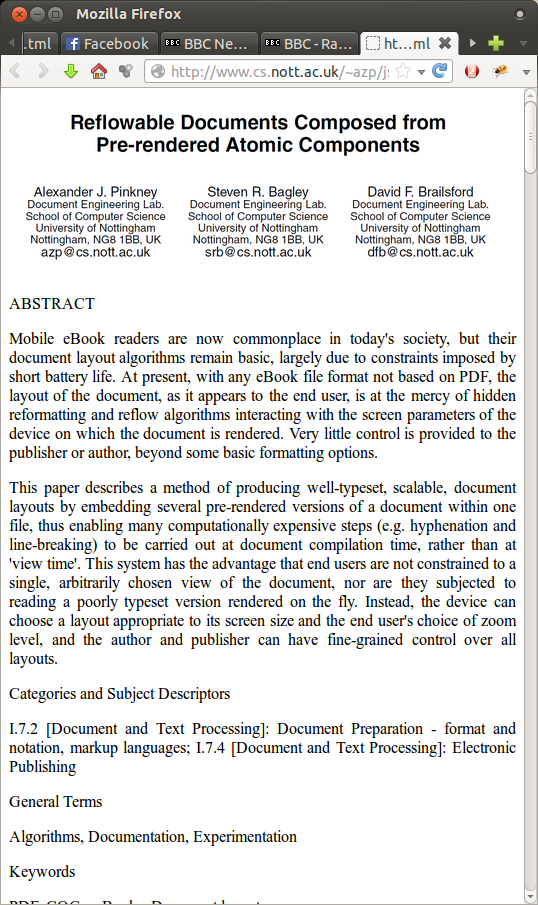
\includegraphics[trim=0in 0in 0in 1.2in, clip=true, width=0.47\textwidth]{gfx/html3}}\hspace{0.01\textwidth}
\fbox{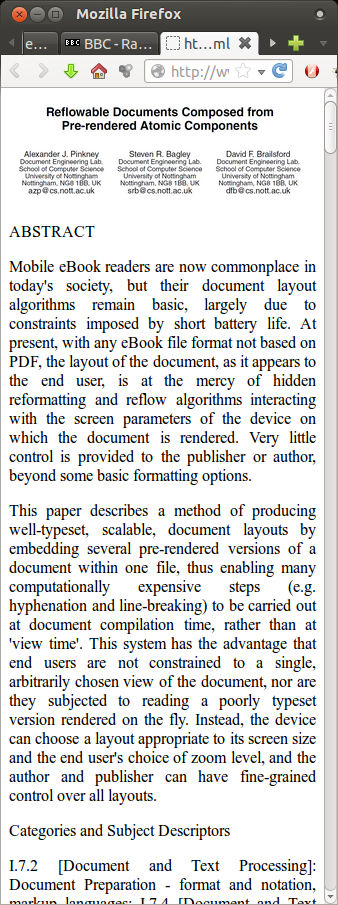
\includegraphics[trim=0in 0in 0in 1.2in, clip=true, width=0.47\textwidth]{gfx/html4}}
\end{center}
\caption[A document laid out by Mozilla Firefox]{\gls{html} version of \cite{Pinkney2011}, as rendered by Mozilla Firefox, scaled to fit multiple screen sizes. Though \gls{html} can stretch to any screen size, it tends to produce typographically inferior results, for example lines that are too long, or line breaking that results in extremely uneven spacing between adjacent lines.}
\label{fig:example-html}
\end{figure}

\todo{Put android screenshots here}
